\documentclass[11pt]{article}
\usepackage[utf8]{inputenc} % LaTeX source encoded as UTF-8
\usepackage[czech]{babel}

\usepackage{graphicx} %graphics files inclusion
\usepackage{amsmath} %advanced maths
\usepackage{amssymb} %additional math symbols
\usepackage{amsfonts}
\usepackage{listings}
\usepackage{hyperref}
\usepackage{color}
\usepackage{graphicx}

\lstset{
	inputencoding=utf8,
	keywords={end,if,for,in,sort, return, and, then},
	keywordstyle=\color{black}\bfseries\em,
}

\begin{document}

\title{2. úloha -- problém batohu (metoda větví a hranic, dynamické programování, FPTAS)}
\author{Ondřej Červenka}
\date{11. 11. 2015}
\maketitle

\section{Specifikace úlohy}

Mějme počet věcí $n \in \mathbb{N}$ a maximální váhu batohu $M \in \mathbb{N}$. \newline Každá věc $i \in \{1, 2, \ldots, n\}$ má určenou váhu $V_i \in \mathbb{N}$ a cenu $C_i \in \mathbb{N}^0$. Úkolem je najít takovou kombinaci věcí, která má co nejvyšší hodnotu a zároveň nepřekračuje maximální váhu batohu $M$.

Problém budeme řešit ve variantě $0/1$, tedy každou věc máme k dispozici pouze jednou. Řešením jsou tedy čísla $\{x_1, x_2, \ldots, x_n\}$, $x_i \in \{0,1\}$ pro která platí $$\sum_{i=1}^n x_iV_i \leq M$$ a zároveň $$\sum_{i=1}^n x_iC_i = max $$ kde $max$ je maximální možná cena.

\section{Řešení}

\subsection{Metoda větví a hranic}

Tento algoritmus rekurzivně prohledává stavový prostor stejně jako rekurzivní algoritmus hrubou silou, je však doplněn o prořezávání stavového prostoru podle ceny. 

Pokud tedy současná cena a cena všech zbývajících předmětů, ze kterých mohu vybírat, nemůže překročit dosud cenu dosud nalezeného nejlepšího řešení, algoritmus ukončí prohledávání aktuální větve rekurze.

\begin{lstlisting}
if current_value + max_value[i] < opt_value then
	return
\end{lstlisting}

Současná cena \verb|current_value| je tedy suma cen předmětů, o kterých bylo v této větvi již rozhodnuto. Pole \verb|max_value| obsahuje předpočítané ceny zbývajících předmětů. Hodnota na indexu $i$ (index předmětu, o kterém právě rozhodujeme) tedy odpovídá $\sum_{j=1}^i C_j$. Hodnota \verb|opt_value| je doposud nejlepší nalezené řešení. 

V rekurzi postupujeme od předmětů s vyšším indexem k předmětům s nižším indexem (začínáme tedy s předmětem $n$). V každém kroku tedy můžeme zkontrolovat cenu všech zbývajících předmětů.

Asymptotická složitost tohoto algoritmu je stále $O(2^n)$, na rozdíl od řešení hrubou silou je však datově závislý. Celý stavový prostor je tedy prohledáván pouze v krajních případech.

Takový případ může být například instance, kde optimální řešení obsahuje všechny (výsledný vektor je $\{x_1 = 1, x_2 = 1, \ldots, x_n = 1\}$), záleží však na pořadí rekurzivních volání (zdali nejprve sestupujeme ve větvi, kde předměty nepřidáváme nebo naopak) a pořadí, ve kterém rozhodujeme o jednotlivých předmětech.

Řešení nalezené tímto algoritmem je vždy optimální.

\subsection{Dynamický algoritmus}

Dynamický algoritmus využívá doposud spočítaných výsledků (zde váhy a ceny batohu) k výpočtu dalšího kroku. Výsledky predchozích kroků jsou ukládány do tabulky, která je algoritmem postupně vyplňována. Vzhledem k potřebě alokovat místo pro tuto tabulku je tedy snížená časová náročnost kompenzována zvýšenou paměťovou náročností.

Algoritmus spočívá v dekompozici problému na podproblémy. Problém je možno dekomponovat podle celkové ceny nebo podle maximální kapacity batohu. Já jsem se rozhodl pro dekompozici podle ceny, neboť ji využijeme i při implementaci FPTAS algoritmu.

Dekompozice podle ceny i váhy vždy najde optimální řešení.

\subsubsection{Dekompozice podle ceny}

Mějme $W(i, c)$ sumu hmotnosti instance, kde bylo rozhodnuto o $i$ věcech, při celkové ceně instance $c$. Toto představuje jedno políčko naší tabulky. Dále platí:

\begin{enumerate}
	\item $i > 0$ 
	\item $W(0,0) = 0$
	\item $\forall c > 0: W(0,c) = \infty$
	\item $W(i+1, c) = min(W(i,c), W(i, c - C_{i+1}) + V_{i+1})$ kde $C_i$ a $V_i$ je cena a váha předmětu $i$
\end{enumerate}

Hodnota $W(i+1, c)$ je tedy definována na základě předchozích hodnot. Samotné řešení je maximální hodnota $c$, kde platí $W(c, n) \leq M$ ($M$ je maximální povolená váha batohu, $n$ znamená, že jsme rozhodli o všech předmětech).

Po nalezení optimální ceny je ještě třeba z tabulky zrekonstruovat vektor řešení. To lze provést tak, že počínaje námi nalezenou optimální cenou $c$ budeme procházet hodnoty v tabulce. Pokud platí $W(c, i) = W(c, i - 1)$, znamená to, že při rozhodnutí o věci $i$ se váha batohu nezměnila, věc tedy není součástí řešení.

Složitost tohoto algoritmu závisí na velikosti tabulky. Tabulku tvoří pole $n \cdot \sum_{i=1}^n C_i$ (suma všech cen je považována jako maximální možná cena řešení). Pokud bychom zavedli $C_m = max(C_1, C_2,\ldots,C_n)$, pak jistě platí $\sum_{i=1}^n C_i \leq n \cdot C_m$. Velikost tabulky bude tedy v nejhorším případě $n^2 \cdot C_m$, z čehož vyplývá, že časová i paměťová složitost algoritmu je $O(n^2 \cdot C_m)$.

\subsection{FPTAS algoritmus}

Dynamický algoritmus běží v pseudopolynomiálním čase. Pokud bychom chtěli skutečně polynomiální algoritmus, musí být ceny předmětů $C_i$ polynomiálně vázané v $n$. 

Při FPTAS algoritmu tedy upravíme jednotlivé ceny předmětů tak, aby byly polynomiálně vázané v $n$ a pomocí dekompozice podle ceny najdeme optimální řešení pro takto upravené předměty.

Schéma algoritmu:
\begin{enumerate}
	\item Zvolíme chybu $\epsilon \in (0,1)$
	\item Mějme $K = \frac{\epsilon C_m}{n}$ kde $C_m = max(C_1, C_2,\ldots,C_n)$
	\item Pro každý předmět $i$ určíme $C'_i = \lfloor \frac{C_i}{K} \rfloor$
	\item Pomocí dekompozice podle ceny spočítáme vektor řešení $\{x_1, x_2,\ldots, x_n\}$ pro ceny $C'_1, C'_2,\ldots,C'_n$
	\item cena přibližného řešení je $APX = \sum_{i=1}^n C_i \cdot x_i$
\end{enumerate}

Takto nalezené řešení nemusí být optimální pro původní ceny předmětů, míru chyby však můžeme určit. Zvolená chyba také ovlivní dobu běhu algoritmu, neboť čím menší zvolíme chybu, tim méně se sníží cena předmětů a tím i velikost tabulky dynamického algoritmu. Cena nalezeného řešení bude alespoň $APX = (1 - \epsilon) \cdot OPT$, kde $\epsilon \in (0,1)$ je zvolená chyba a $OPT$ je cena optimálního řešení.\cite{kate}

\section{Výsledky}

\subsection{Podmínky měření}

Algoritmy byly implementovány v C a kompilovány pomocí gcc 5.1.1. Při kompilaci nebyly použity žádné optimalizační přepínače. Program byl zkompilován a spouštěn na operačním systému GNU/Linux (Fedora) 64bit s verzí jádra 4.2.5. Procesor počítače je Intel Core i7-4510U s frekvencí 3.1 GHz.

Výsledné časy běhu exaktních algoritmů a FPTAS algoritmu pro instance velikosti 4 a 10 byly získány průměrem z 10 000 běhů. 

Časy běhu byly získány pomocí funkce $clock()$ z knihovny $time.h$.

\subsection{Časy exaktních algoritmů}

\begin{figure}[h!]
	\centering
    	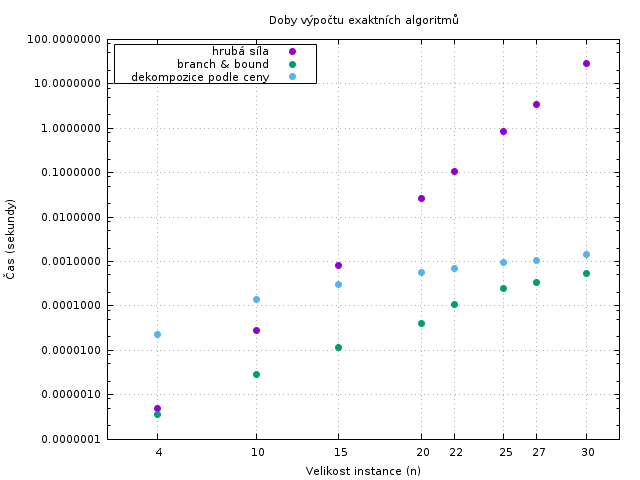
\includegraphics[width=0.8\textwidth]{exact_times.png}
    	\caption{Grafy časů pro exaktní algoritmy}
	\label{fig:exact_times}
\end{figure}

Z grafu \ref{fig:exact_times} tedy můžeme vidět, že prořezávání stavového prostoru dosahuje lepších výsledků než řešení hrubou silou i v malých instancích. Složitost je stále $O(2^n)$, není tedy možné, aby algoritmus prořezávající stavový prostor byl horší, než ten který ho prohledává celý. 

Oproti tomu dynamický algoritmus využívající dekompozici podle ceny vykazuje pro některá $n$ horší výsledky než rešení hrubou silou. To je dáno tím, že kromě $n$ je závislý i na cenách jednotlivých předmětů. 

U našich testovacích dat jsou ceny relativně konzistentí (pohybují se v řádu desítek až stovek pro všechny instance), závislost se tedy projeví spíše u malých instancí. Obecně by však mohla být vychýlená jakákoliv instance, pokud by se její ceny významě lišily od ostatních.

\subsection{Časy FPTAS algoritmu}

Na grafu \ref{fig:apx_times} můžeme vidět, že časy FPTAS algoritmu odpovídají časům dynamického algoritmu z grafu \ref{fig:exact_times}, jsou však posunuty po ose $y$ dolů, v závislosti na zvolené chybě $\epsilon$. 

Můžeme také pozorovat, že s zvyšující se chybou zrychlení algoritmu (oproti menší chybě) klesá (rozdíl mezi časy výpočtu pro $\epsilon = 0.1$ a $\epsilon = 0.3$ je přibližně trojnásobný, kdežto rozdíl mezi $\epsilon = 0.6$ a $\epsilon = 0.9$ je zhruba 50\%).

\begin{figure}[h!]
	\centering
    	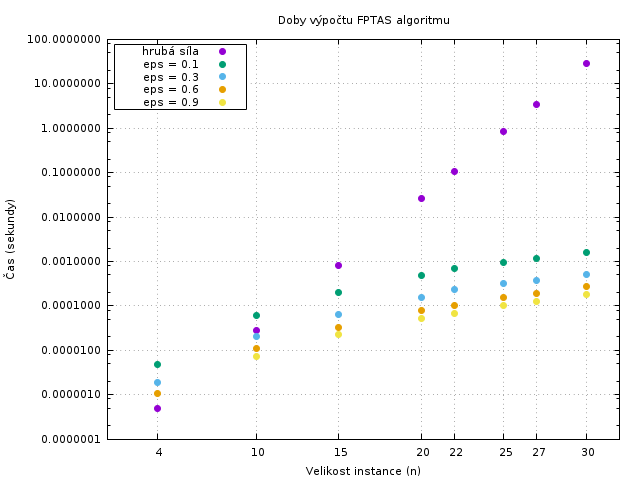
\includegraphics[width=0.8\textwidth]{apx_times.png}
    	\caption{Grafy časů FPTAS algoritmu}
	\label{fig:apx_times}
\end{figure}

\subsection{Chyba FPTAS algoritmu}

Relativní chyba byla spočítána pomocí vzorce $\epsilon_{rel} = (OPT - APX_\epsilon) / OPT$, kde $APX$ je cena přibližného řešení se zvolenou chybou $\epsilon$ a $OPT$ cena optimálního řešení. 

Z grafu \ref{fig:apx_error} lze vidět, že relativní chyba rychle roste se zvyšujícím se $\epsilon$, pro větší velikost instanci $n$ naopak mírně klesá.

\begin{figure}[h!]
	\centering
    	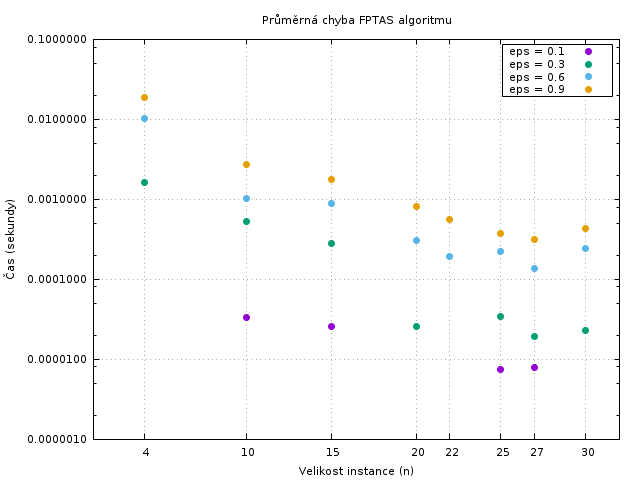
\includegraphics[width=0.8\textwidth]{apx_error.png}
    	\caption{Grafy průměrné chyby FPTAS algoritmu}
	\label{fig:apx_error}
\end{figure}

\begin{figure}[h!]
	\centering
    	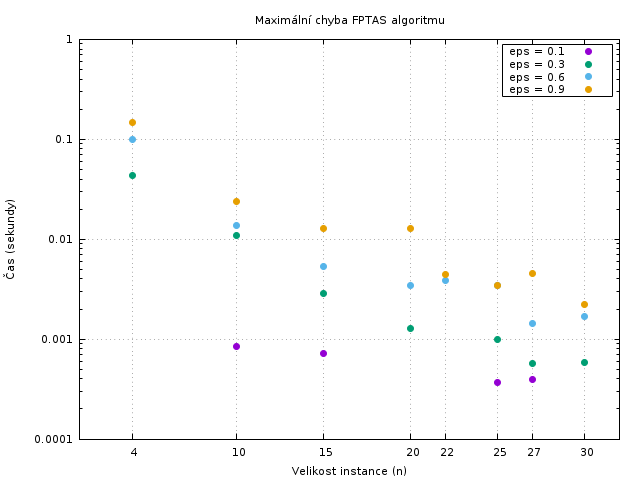
\includegraphics[width=0.8\textwidth]{apx_max_error.png}
    	\caption{Grafy maximální chyby FPTAS algoritmu}
	\label{fig:apx_max_error}
\end{figure}

\newpage

\section{Závěr}

Při měření mě překvapila rychlost výpočtu při prořezávání stavového prostoru, vzhledem k poměrně silné datové závislosti by však bylo vhodné provést měření na dalších datech. 

Stejně tak platí v případě algoritmu využívajícího dekompozici podle cen, neboť rozmezí cen v jednotlivých instancích v testovacích datech se nijak výrazně neliší. Dekompozice podle váhy by pravděpodobně přinesla podobné výsledky, neboť v testovacích dataech $M$ také roste úměrně s $n$.

U FPTAS algoritmu se ukázalo, že zvyšovat $\epsilon$ za účelem zrychlení výpočtu má smysl jen do určité meze.

\bibliographystyle{csn690}
\bibliography{mybibliographyfile}

\end{document}
